\documentclass{article}
\usepackage{xcolor}
\usepackage{graphicx}
\usepackage{float}
\usepackage{tikz}
\usepackage{parskip}
\usepackage{amsmath}
\usepackage{amsthm}
\usepackage{amssymb}
\usepackage{mathtools}
\usepackage{fancyhdr}
\usepackage[%paperheight = 59.4cm,
            %paperwidth = 42cm,
            %includehead,
            nomarginpar,
            textwidth=15cm,
            headheight=10mm]{geometry}


\begin{document}
 
\pagestyle{fancy}
%\fancyhead{}\fancyfoot{}

\fancyhf[OHC]{Christopher Munoz WRH3 Optimization}
\textbf{Problem 4.2:} \\
In this problem we explore descent directions for the linear function $f(x) = x_1 - 2x_2 + 3x_3$ and determine whether our solutions depend on the value of x. Let us consider the gradient of our linear function:
\begin{align*}
    \nabla f(x) = \begin{bmatrix} 1 \\ -2 \\ 3 \end{bmatrix}
\end{align*}
We let d be the dscent direction

\textbf{Problem 4.3:} Consider the following problem: 
\begin{align*}
    \text{minimize} &\null \quad f(x) = -x_1 - x_2 \\ 
    \text{subject to} &\null \quad x_1 + x_2 \leq 2 \\
     &\null \quad x_1, x_2 \geq 0
\end{align*}
We will do the following: \newline \setlength\parindent{24pt}  
\indent \{i\} Determine the feasible directions at  $x = (0,0)^T, (0,1)^T, (1,1)^T$ and $(0,2)^T$ \newline 
\indent \{ii\} Determine whether there exist feasible descent direction at these points, and hence determine which (if any) of the point can be local minimizers. 
\newline 
\begin{figure}[H]
    \centering
    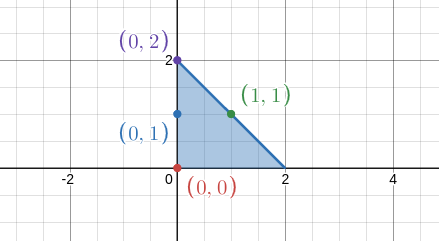
\includegraphics[scale = 0.40]{desmos2.png}
\end{figure}
\indent \textbf{\{i\}} Solution, below we let $p$ be a set of vectors.
\begin{align*}
    \bar{x} = (0,0)^T: &\null \quad \{p \in \mathbb{R}^2 | p_1 \geq 0, p_2 \geq 0 \} \\
    \bar{x} = (0,1)^T: &\null \quad \{p \in \mathbb{R}^2 | p_1 \geq 0, p_1 \leq 1 \} \\
    \bar{x} = (1,1)^T: &\null \quad \{p \in \mathbb{R}^2 | p_1 + p_2 \leq 0 \} \\
    \bar{x} = (0,2)^T: &\null \quad \{p \in \mathbb{R}^2 | p_1 + p_2 \leq 2 \}, \text{ where } \{p_2 \leq 0\}\\
\end{align*}
\indent \textbf{\{ii\}} \newline For the point $(0,0)^T$, every direction $p_1 \geq 0$ and $p_2 \geq 0$ is a feasible descent direction. Its not a local minimizer. \newline
For the point $(0,1)^T$, there are feasible directions if $0 \leq p_1 \leq 1$ and $p_2 $, not a local minimizer. \newline
For point $(1,1)$, there are no feasible directions, this is actually the global minimizer \newline
For point $(0,2)$ there are no feasible directions

\textbf{Problem 6.4:}

\end{document}
